\documentclass{standalone}
\usepackage{tikz}
\usetikzlibrary{patterns}
\usetikzlibrary{positioning}
\usetikzlibrary{patterns, positioning}
\usetikzlibrary{shapes.misc}
\usepackage[outline]{contour}
\contourlength{1.5pt} 
\usepackage[sfdefault]{ClearSans}

\begin{document}
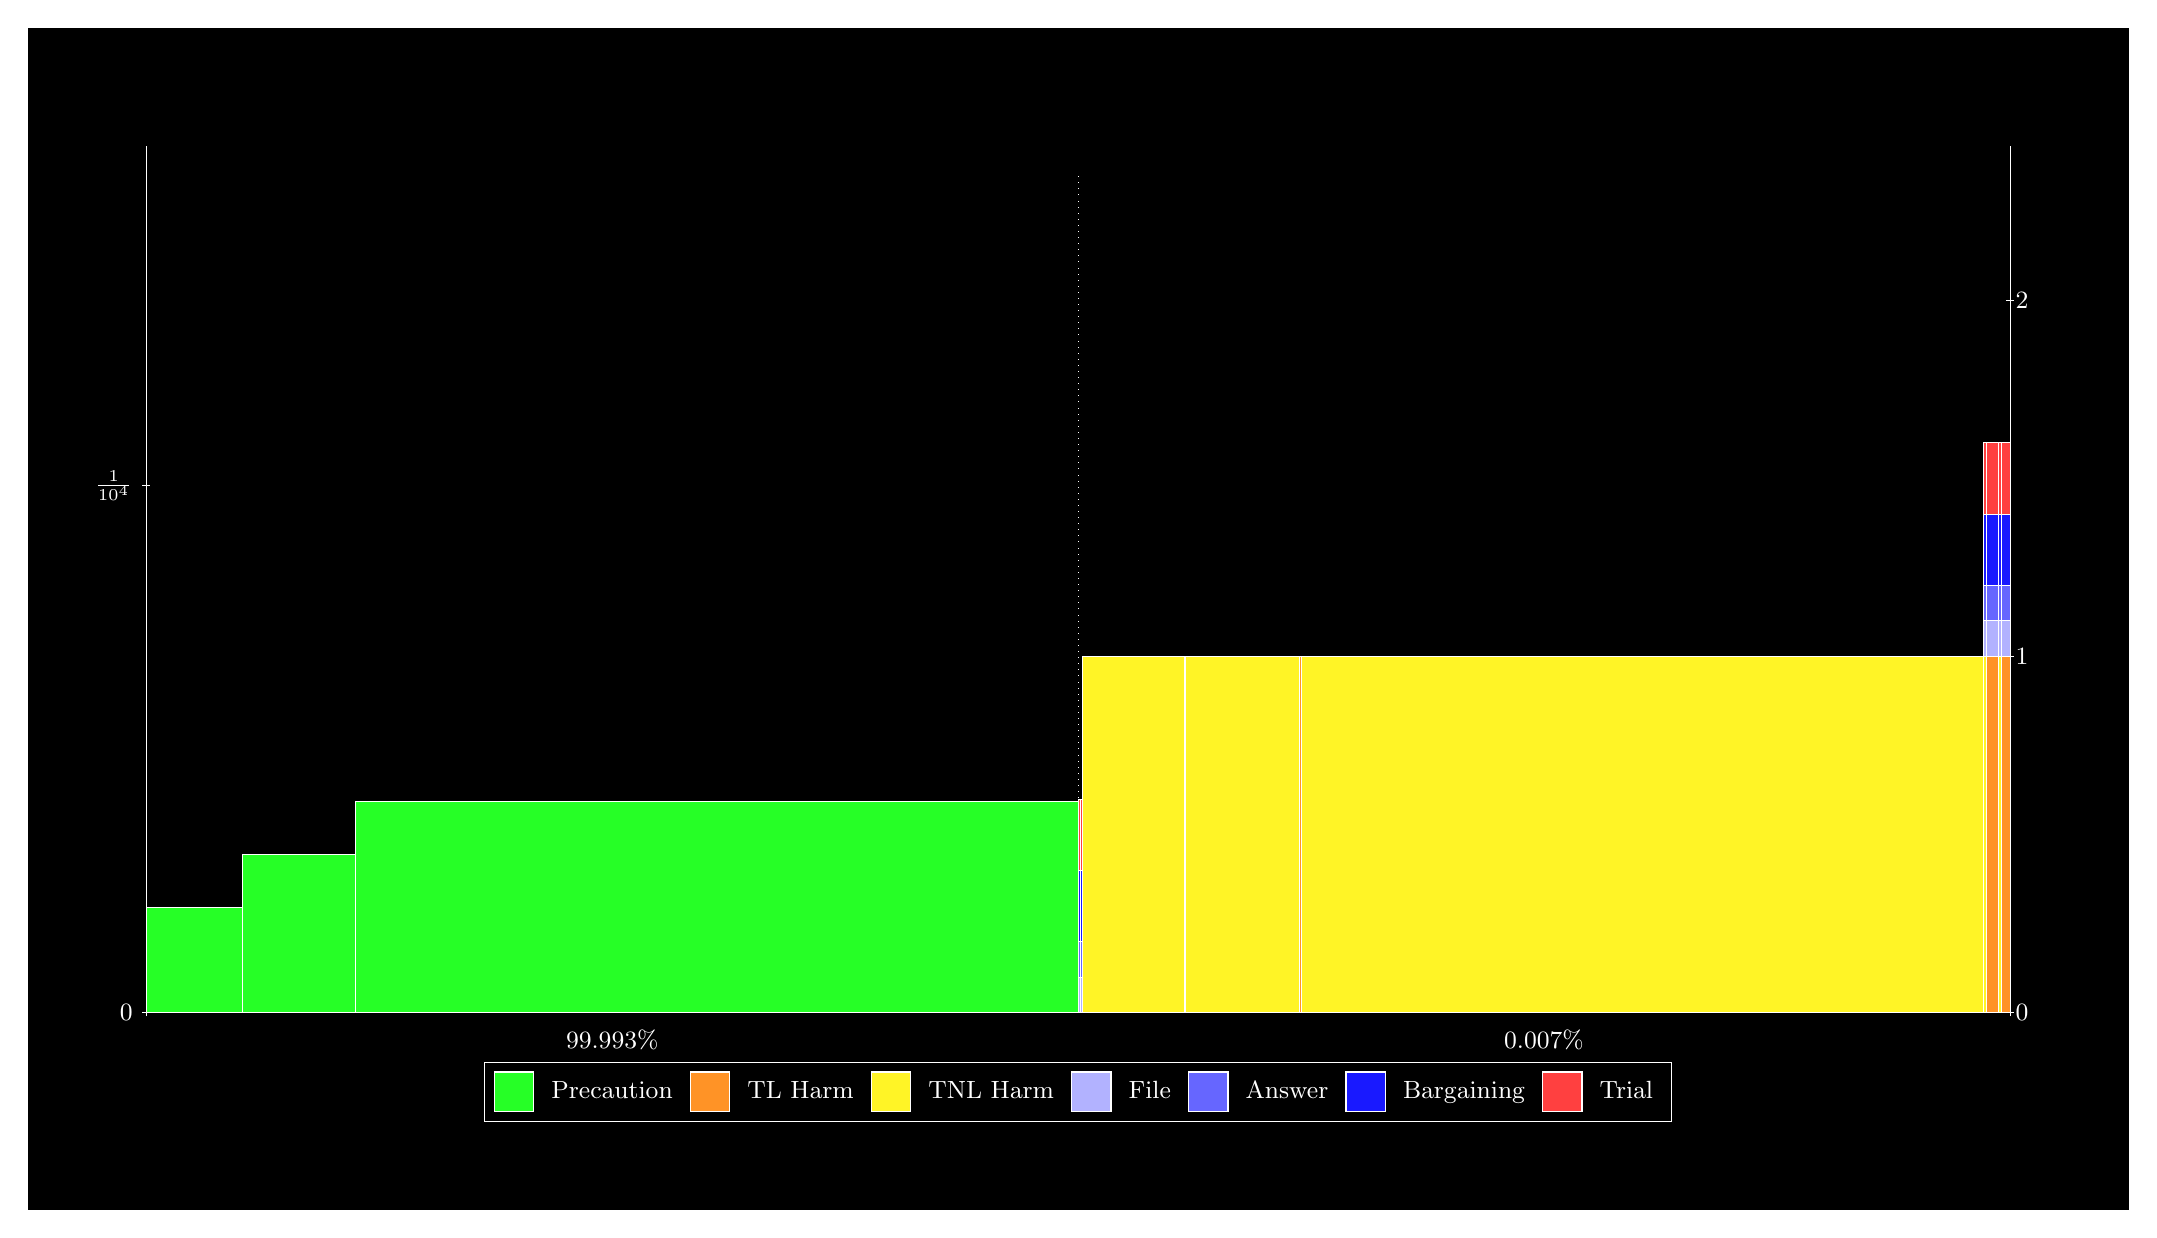
\begin{tikzpicture}
\draw[fill=black] (0,0) rectangle (26.667,15);
\draw[fill=green!85,draw=white,very thin] (1.5,2.5) rectangle (2.7157,3.8381);
\draw[fill=green!85,draw=white,very thin] (2.7157,2.5) rectangle (4.1478,4.5071);
\draw[fill=green!85,draw=white,very thin] (4.1478,2.5) rectangle (13.333,5.1761);
\draw[fill=green!85,draw=white,very thin] (13.333,2.5) rectangle (13.358,2.5001);
\draw[fill=blue!30,draw=white,very thin] (13.333,2.5001) rectangle (13.358,2.9523);
\draw[fill=blue!60,draw=white,very thin] (13.333,2.9523) rectangle (13.358,3.4046);
\draw[fill=blue!90,draw=white,very thin] (13.333,3.4046) rectangle (13.358,4.309);
\draw[fill=red!75,draw=white,very thin] (13.333,4.309) rectangle (13.358,5.2135);
\draw[fill=green!85,draw=white,very thin] (13.358,2.5) rectangle (13.38,2.5001);
\draw[fill=blue!30,draw=white,very thin] (13.358,2.5001) rectangle (13.38,2.9524);
\draw[fill=blue!60,draw=white,very thin] (13.358,2.9524) rectangle (13.38,3.4046);
\draw[fill=blue!90,draw=white,very thin] (13.358,3.4046) rectangle (13.38,4.3091);
\draw[fill=red!75,draw=white,very thin] (13.358,4.3091) rectangle (13.38,5.2136);
\draw[fill=green!85,draw=white,very thin] (13.38,2.5) rectangle (14.678,2.5001);
\draw[fill=yellow!85,draw=white,very thin] (13.38,2.5001) rectangle (14.678,7.0225);
\draw[fill=green!85,draw=white,very thin] (14.678,2.5) rectangle (14.7,2.5001);
\draw[fill=orange!85,draw=white,very thin] (14.678,2.5001) rectangle (14.7,7.0225);
\draw[fill=green!85,draw=white,very thin] (14.7,2.5) rectangle (16.142,2.5001);
\draw[fill=yellow!85,draw=white,very thin] (14.7,2.5001) rectangle (16.142,7.0225);
\draw[fill=green!85,draw=white,very thin] (16.142,2.5) rectangle (16.166,2.5001);
\draw[fill=orange!85,draw=white,very thin] (16.142,2.5001) rectangle (16.166,7.0225);
\draw[fill=green!85,draw=white,very thin] (16.166,2.5) rectangle (24.835,2.5002);
\draw[fill=yellow!85,draw=white,very thin] (16.166,2.5002) rectangle (24.835,7.0226);
\draw[fill=green!85,draw=white,very thin] (24.835,2.5) rectangle (24.871,2.5001);
\draw[fill=yellow!85,draw=white,very thin] (24.835,2.5001) rectangle (24.871,7.0225);
\draw[fill=blue!30,draw=white,very thin] (24.835,7.0225) rectangle (24.871,7.4747);
\draw[fill=blue!60,draw=white,very thin] (24.835,7.4747) rectangle (24.871,7.9269);
\draw[fill=blue!90,draw=white,very thin] (24.835,7.9269) rectangle (24.871,8.8314);
\draw[fill=red!75,draw=white,very thin] (24.835,8.8314) rectangle (24.871,9.7359);
\draw[fill=green!85,draw=white,very thin] (24.871,2.5) rectangle (25.023,2.5001);
\draw[fill=orange!85,draw=white,very thin] (24.871,2.5001) rectangle (25.023,7.0225);
\draw[fill=blue!30,draw=white,very thin] (24.871,7.0225) rectangle (25.023,7.4747);
\draw[fill=blue!60,draw=white,very thin] (24.871,7.4747) rectangle (25.023,7.9269);
\draw[fill=blue!90,draw=white,very thin] (24.871,7.9269) rectangle (25.023,8.8314);
\draw[fill=red!75,draw=white,very thin] (24.871,8.8314) rectangle (25.023,9.7359);
\draw[fill=green!85,draw=white,very thin] (25.023,2.5) rectangle (25.052,2.5001);
\draw[fill=yellow!85,draw=white,very thin] (25.023,2.5001) rectangle (25.052,7.0225);
\draw[fill=blue!30,draw=white,very thin] (25.023,7.0225) rectangle (25.052,7.4747);
\draw[fill=blue!60,draw=white,very thin] (25.023,7.4747) rectangle (25.052,7.927);
\draw[fill=blue!90,draw=white,very thin] (25.023,7.927) rectangle (25.052,8.8315);
\draw[fill=red!75,draw=white,very thin] (25.023,8.8315) rectangle (25.052,9.7359);
\draw[fill=green!85,draw=white,very thin] (25.052,2.5) rectangle (25.167,2.5001);
\draw[fill=orange!85,draw=white,very thin] (25.052,2.5001) rectangle (25.167,7.0225);
\draw[fill=blue!30,draw=white,very thin] (25.052,7.0225) rectangle (25.167,7.4747);
\draw[fill=blue!60,draw=white,very thin] (25.052,7.4747) rectangle (25.167,7.927);
\draw[fill=blue!90,draw=white,very thin] (25.052,7.927) rectangle (25.167,8.8315);
\draw[fill=red!75,draw=white,very thin] (25.052,8.8315) rectangle (25.167,9.7359);
\draw[white,very thin] (1.5,2.5) -- (1.5,13.5);
\draw[white,very thin] (1.45,2.5) -- (1.55,2.5);
\node[font=\small,text=white, anchor=east] at (1.45, 2.5) {0};
\draw[white,very thin] (1.45,9.1903) -- (1.55,9.1903);
\node[font=\small,text=white, anchor=east] at (1.45, 9.1903) {$\frac{1}{10^{4}}$};

\draw[white,dotted,very thin] (13.333,2.83) -- (13.333,13.17);
\draw[white,very thin] (25.167,2.5) -- (25.167,13.5);
\draw[white,very thin] (25.117,2.5) -- (25.217,2.5);
\node[font=\small,text=white, anchor=west] at (25.117, 2.5) {0};
\draw[white,very thin] (25.117,7.0224) -- (25.217,7.0224);
\node[font=\small,text=white, anchor=west] at (25.117, 7.0224) {1};
\draw[white,very thin] (25.117,11.545) -- (25.217,11.545);
\node[font=\small,text=white, anchor=west] at (25.117, 11.545) {2};

\draw[white,very thin] (1.5,2.5) -- (25.167,2.5);
\draw[white,very thin] (1.5,2.45) -- (1.5,2.55);
\node[font=\small,text=white, anchor=north] at (1.5, 2.45) {};
\draw[white,very thin] (25.167,2.45) -- (25.167,2.55);
\node[font=\small,text=white, anchor=north] at (25.167, 2.45) {};

\node[font=\small,text=white,anchor=south] at (7.4167, 1.9) {99.993\%};
\node[font=\small,text=white,anchor=south] at (19.25, 1.9) {0.007\%};
\draw (13.3333,2.5) node (B) {};
\begin{scope}[align=center]
\matrix[scale=0.5,draw=white,below=0.5cm of B,nodes={draw},column sep=0.1cm]{
\node[rectangle,draw,minimum width=0.5cm,minimum height=0.5cm,fill=green!85]{}; & \node[draw=none,font=\small,text=white]{Precaution}; &
\node[rectangle,draw,minimum width=0.5cm,minimum height=0.5cm,fill=orange!85]{}; & \node[draw=none,font=\small,text=white]{TL Harm}; &
\node[rectangle,draw,minimum width=0.5cm,minimum height=0.5cm,fill=yellow!85]{}; & \node[draw=none,font=\small,text=white]{TNL Harm}; &
\node[rectangle,draw,minimum width=0.5cm,minimum height=0.5cm,fill=blue!30]{}; & \node[draw=none,font=\small,text=white]{File}; &
\node[rectangle,draw,minimum width=0.5cm,minimum height=0.5cm,fill=blue!60]{}; & \node[draw=none,font=\small,text=white]{Answer}; &
\node[rectangle,draw,minimum width=0.5cm,minimum height=0.5cm,fill=blue!90]{}; & \node[draw=none,font=\small,text=white]{Bargaining}; &
\node[rectangle,draw,minimum width=0.5cm,minimum height=0.5cm,fill=red!75]{}; & \node[draw=none,font=\small,text=white]{Trial}; \\\\
};\end{scope}

\end{tikzpicture}
\end{document}